% Gerado automaticamente. No preambulo do documento use:
% \usepackage{pgfplots}
% \pgfplotsset{compat=1.18}
\definecolor{plotblue}{HTML}{2563EB}
\definecolor{plotorange}{HTML}{D97706}
\definecolor{plotgreen}{HTML}{059669}
\definecolor{plotpurple}{HTML}{7C3AED}
\definecolor{plotgray}{HTML}{374151}
\definecolor{plotred}{HTML}{DC2626}
\definecolor{plotteal}{HTML}{0F766E}
\definecolor{plotslate}{HTML}{64748B}

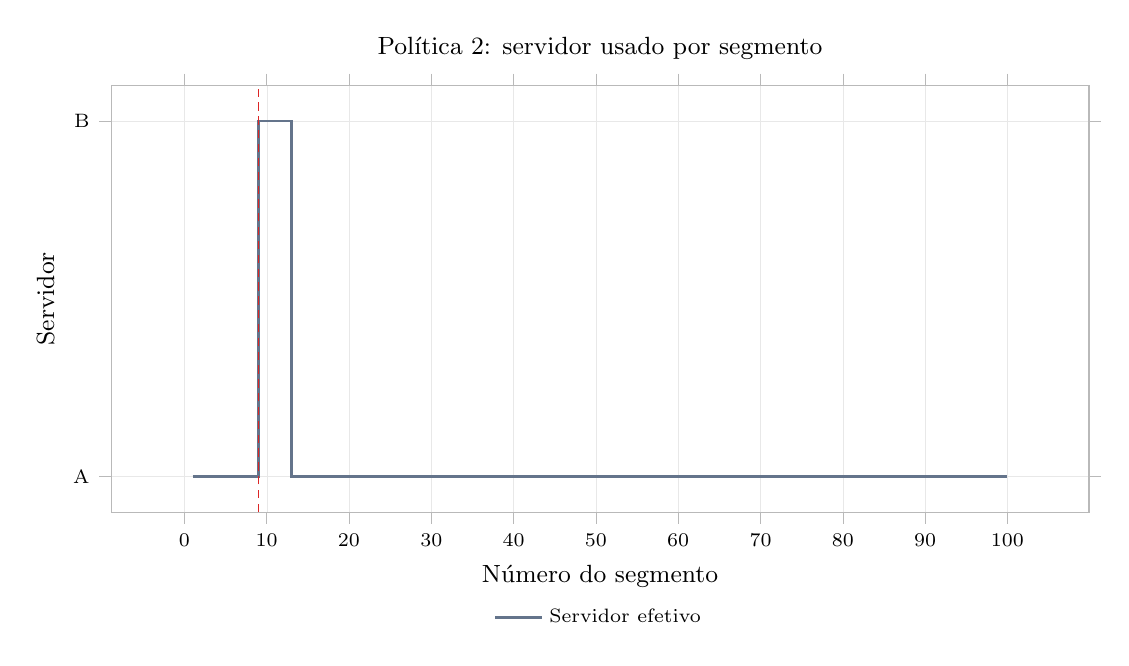
\begin{tikzpicture}
\begin{axis}[
    title={Política 2: servidor usado por segmento},
    xlabel={Número do segmento},
    ylabel={Servidor},
    width=14cm,
    height=7cm,
    grid=major,
    grid style={line width=.12pt, draw=gray!18},
    axis line style={draw=gray!55},
    tick style={draw=gray!55},
    tick align=outside,
    title style={font=\small},
    label style={font=\small},
    tick label style={font=\scriptsize},
    legend cell align={left},
    legend style={at={(0.5,-0.20)}, anchor=north, legend columns=1, draw=none, font=\scriptsize},
    ytick={0,1},
    yticklabels={{A},{B}},
    ymin=-0.1,
    ymax=1.1
]
\addplot+[plotslate, const plot, line width=1.05pt, mark=none] coordinates {
(1,0)
(2,0)
(3,0)
(4,0)
(5,0)
(6,0)
(7,0)
(8,0)
(9,1)
(10,1)
(11,1)
(12,1)
(13,0)
(14,0)
(15,0)
(16,0)
(17,0)
(18,0)
(19,0)
(20,0)
(21,0)
(22,0)
(23,0)
(24,0)
(25,0)
(26,0)
(27,0)
(28,0)
(29,0)
(30,0)
(31,0)
(32,0)
(33,0)
(34,0)
(35,0)
(36,0)
(37,0)
(38,0)
(39,0)
(40,0)
(41,0)
(42,0)
(43,0)
(44,0)
(45,0)
(46,0)
(47,0)
(48,0)
(49,0)
(50,0)
(51,0)
(52,0)
(53,0)
(54,0)
(55,0)
(56,0)
(57,0)
(58,0)
(59,0)
(60,0)
(61,0)
(62,0)
(63,0)
(64,0)
(65,0)
(66,0)
(67,0)
(68,0)
(69,0)
(70,0)
(71,0)
(72,0)
(73,0)
(74,0)
(75,0)
(76,0)
(77,0)
(78,0)
(79,0)
(80,0)
(81,0)
(82,0)
(83,0)
(84,0)
(85,0)
(86,0)
(87,0)
(88,0)
(89,0)
(90,0)
(91,0)
(92,0)
(93,0)
(94,0)
(95,0)
(96,0)
(97,0)
(98,0)
(99,0)
(100,0)
};
\addlegendentry{Servidor efetivo}
\addplot+[plotred, line width=0.65pt, densely dashed, mark=none, forget plot] coordinates {(9,-0.1) (9,1.1)};
\end{axis}
\end{tikzpicture}
